\documentclass[12pt, letterpaper]{article}

% ── Paquetes ─────────────────────────────────────────────────────────────────
\usepackage[utf8]{inputenc}
\usepackage[T1]{fontenc}
\usepackage[spanish]{babel}
\usepackage{geometry}
\usepackage{graphicx}
\usepackage{booktabs}
\usepackage{hyperref}
\usepackage{float}
\usepackage{caption}
\usepackage{subcaption}
\usepackage{enumitem}
\usepackage{parskip}
\usepackage{titlesec}
\usepackage{fancyhdr}
\usepackage{xcolor}
\usepackage{lmodern}
\usepackage{microtype}
\usepackage{csquotes}
\usepackage{listings}
\lstset{
  literate={á}{{\'a}}1 {é}{{\'e}}1 {í}{{\'i}}1 {ó}{{\'o}}1 {ú}{{\'u}}1
           {Á}{{\'A}}1 {É}{{\'E}}1 {Í}{{\'I}}1 {Ó}{{\'O}}1 {Ú}{{\'U}}1
           {ñ}{{\~n}}1 {Ñ}{{\~N}}1 {ü}{{\"u}}1 {Ü}{{\"U}}1
}

% ── Geometría ─────────────────────────────────────────────────────────────────
\geometry{
  top=2.5cm, bottom=2.5cm,
  left=2.5cm, right=2.5cm
}
\setlength{\headheight}{13.6pt}

% ── Hyperref ──────────────────────────────────────────────────────────────────
\hypersetup{
  colorlinks=true,
  linkcolor=black,
  urlcolor=blue!70!black,
  citecolor=black
}

% ── Encabezado / pie de página ────────────────────────────────────────────────
\pagestyle{fancy}
\fancyhf{}
\fancyhead[L]{\small Visualización de Datos -- Semestre I, 2026}
\fancyhead[R]{\small Tarea 2}
\fancyfoot[C]{\thepage}
\renewcommand{\headrulewidth}{0.4pt}

% ── Título de secciones ───────────────────────────────────────────────────────
\titleformat{\section}{\large\bfseries}{}{0em}{\thesection.\quad}
\titleformat{\subsection}{\normalsize\bfseries}{}{0em}{\thesubsection.\quad}

% ─────────────────────────────────────────────────────────────────────────────
\begin{document}

% ── Portada ───────────────────────────────────────────────────────────────────
\begin{titlepage}
  \centering
  \vspace*{1.5cm}

  {\Large\bfseries Universidad Técnica Federico Santa María}\\[0.3cm]
  {\large Departamento de Informática}\\[0.2cm]
  {\large Visualización de Datos -- Semestre I, 2026}

  \vspace{1.5cm}
  \rule{\linewidth}{0.5pt}\\[0.4cm]
  {\LARGE\bfseries Tarea 2: Encuestas e Infografías}\\[0.2cm]
  {\large Macrotema: \textit{Muerte} -- Percepciones sobre tasas de suicidio a nivel mundial}
  \rule{\linewidth}{0.5pt}

  \vspace{1.5cm}

  \begin{tabular}{ll}
    \textbf{Integrante 1:} & Alexis Mellis \\[0.2cm]
    \textbf{Integrante 2:} & Andres Aguila \\
  \end{tabular}

  \vspace{1cm}

  \begin{tabular}{ll}
    \textbf{Profesor:}  & José Luis Martí Lara \\[0.3cm]
    \textbf{Ayudantes:}   & Fernanda Araya Zárate \\
                          & Carlos Arévalo Guajardo \\
  \end{tabular}

  \vfill

\end{titlepage}

% ── Índice ────────────────────────────────────────────────────────────────────
\tableofcontents
\newpage

% ─────────────────────────────────────────────────────────────────────────────
\section{Introducción}

% TODO: Escribir introducción de la tarea 2. Contexto de la encuesta,
%       tema abordado y estructura del informe.

% ─────────────────────────────────────────────────────────────────────────────
\section{Encuesta}

\subsection{Descripción y preguntas}

% TODO: Describir brevemente la encuesta (plataforma usada, tema,
%       número de preguntas). Listar las preguntas aquí.

\subsection{Difusión y respuestas obtenidas}

% TODO: Indicar cómo se difundió la encuesta y cuántas respuestas se obtuvieron.
%       Insertar pantallazo que demuestre las 20+ respuestas.

\begin{figure}[H]
  \centering
  % 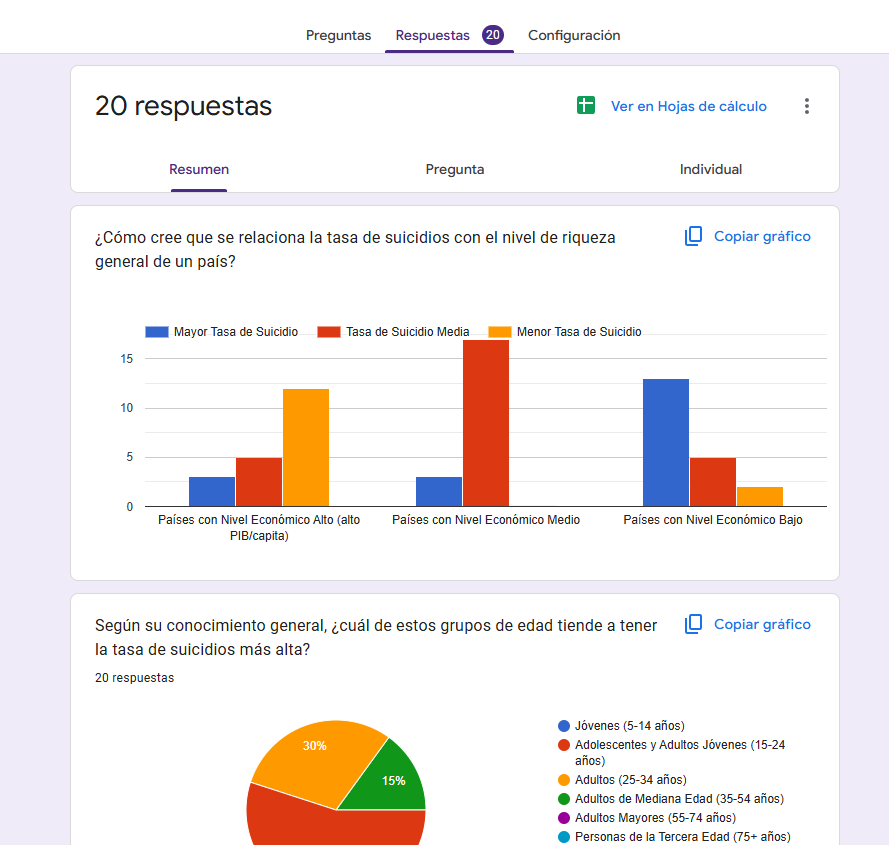
\includegraphics[width=0.7\textwidth]{figures/respuestas.png}
  \caption{Pantallazo del formulario mostrando el total de respuestas obtenidas.}
  \label{fig:respuestas}
\end{figure}

\subsection{Dataset generado}

% TODO: Describir brevemente las variables del CSV descargado.

% ─────────────────────────────────────────────────────────────────────────────
\section{Infografía grupal}

% TODO: Insertar la infografía grupal final.

\begin{figure}[H]
  \centering
  % 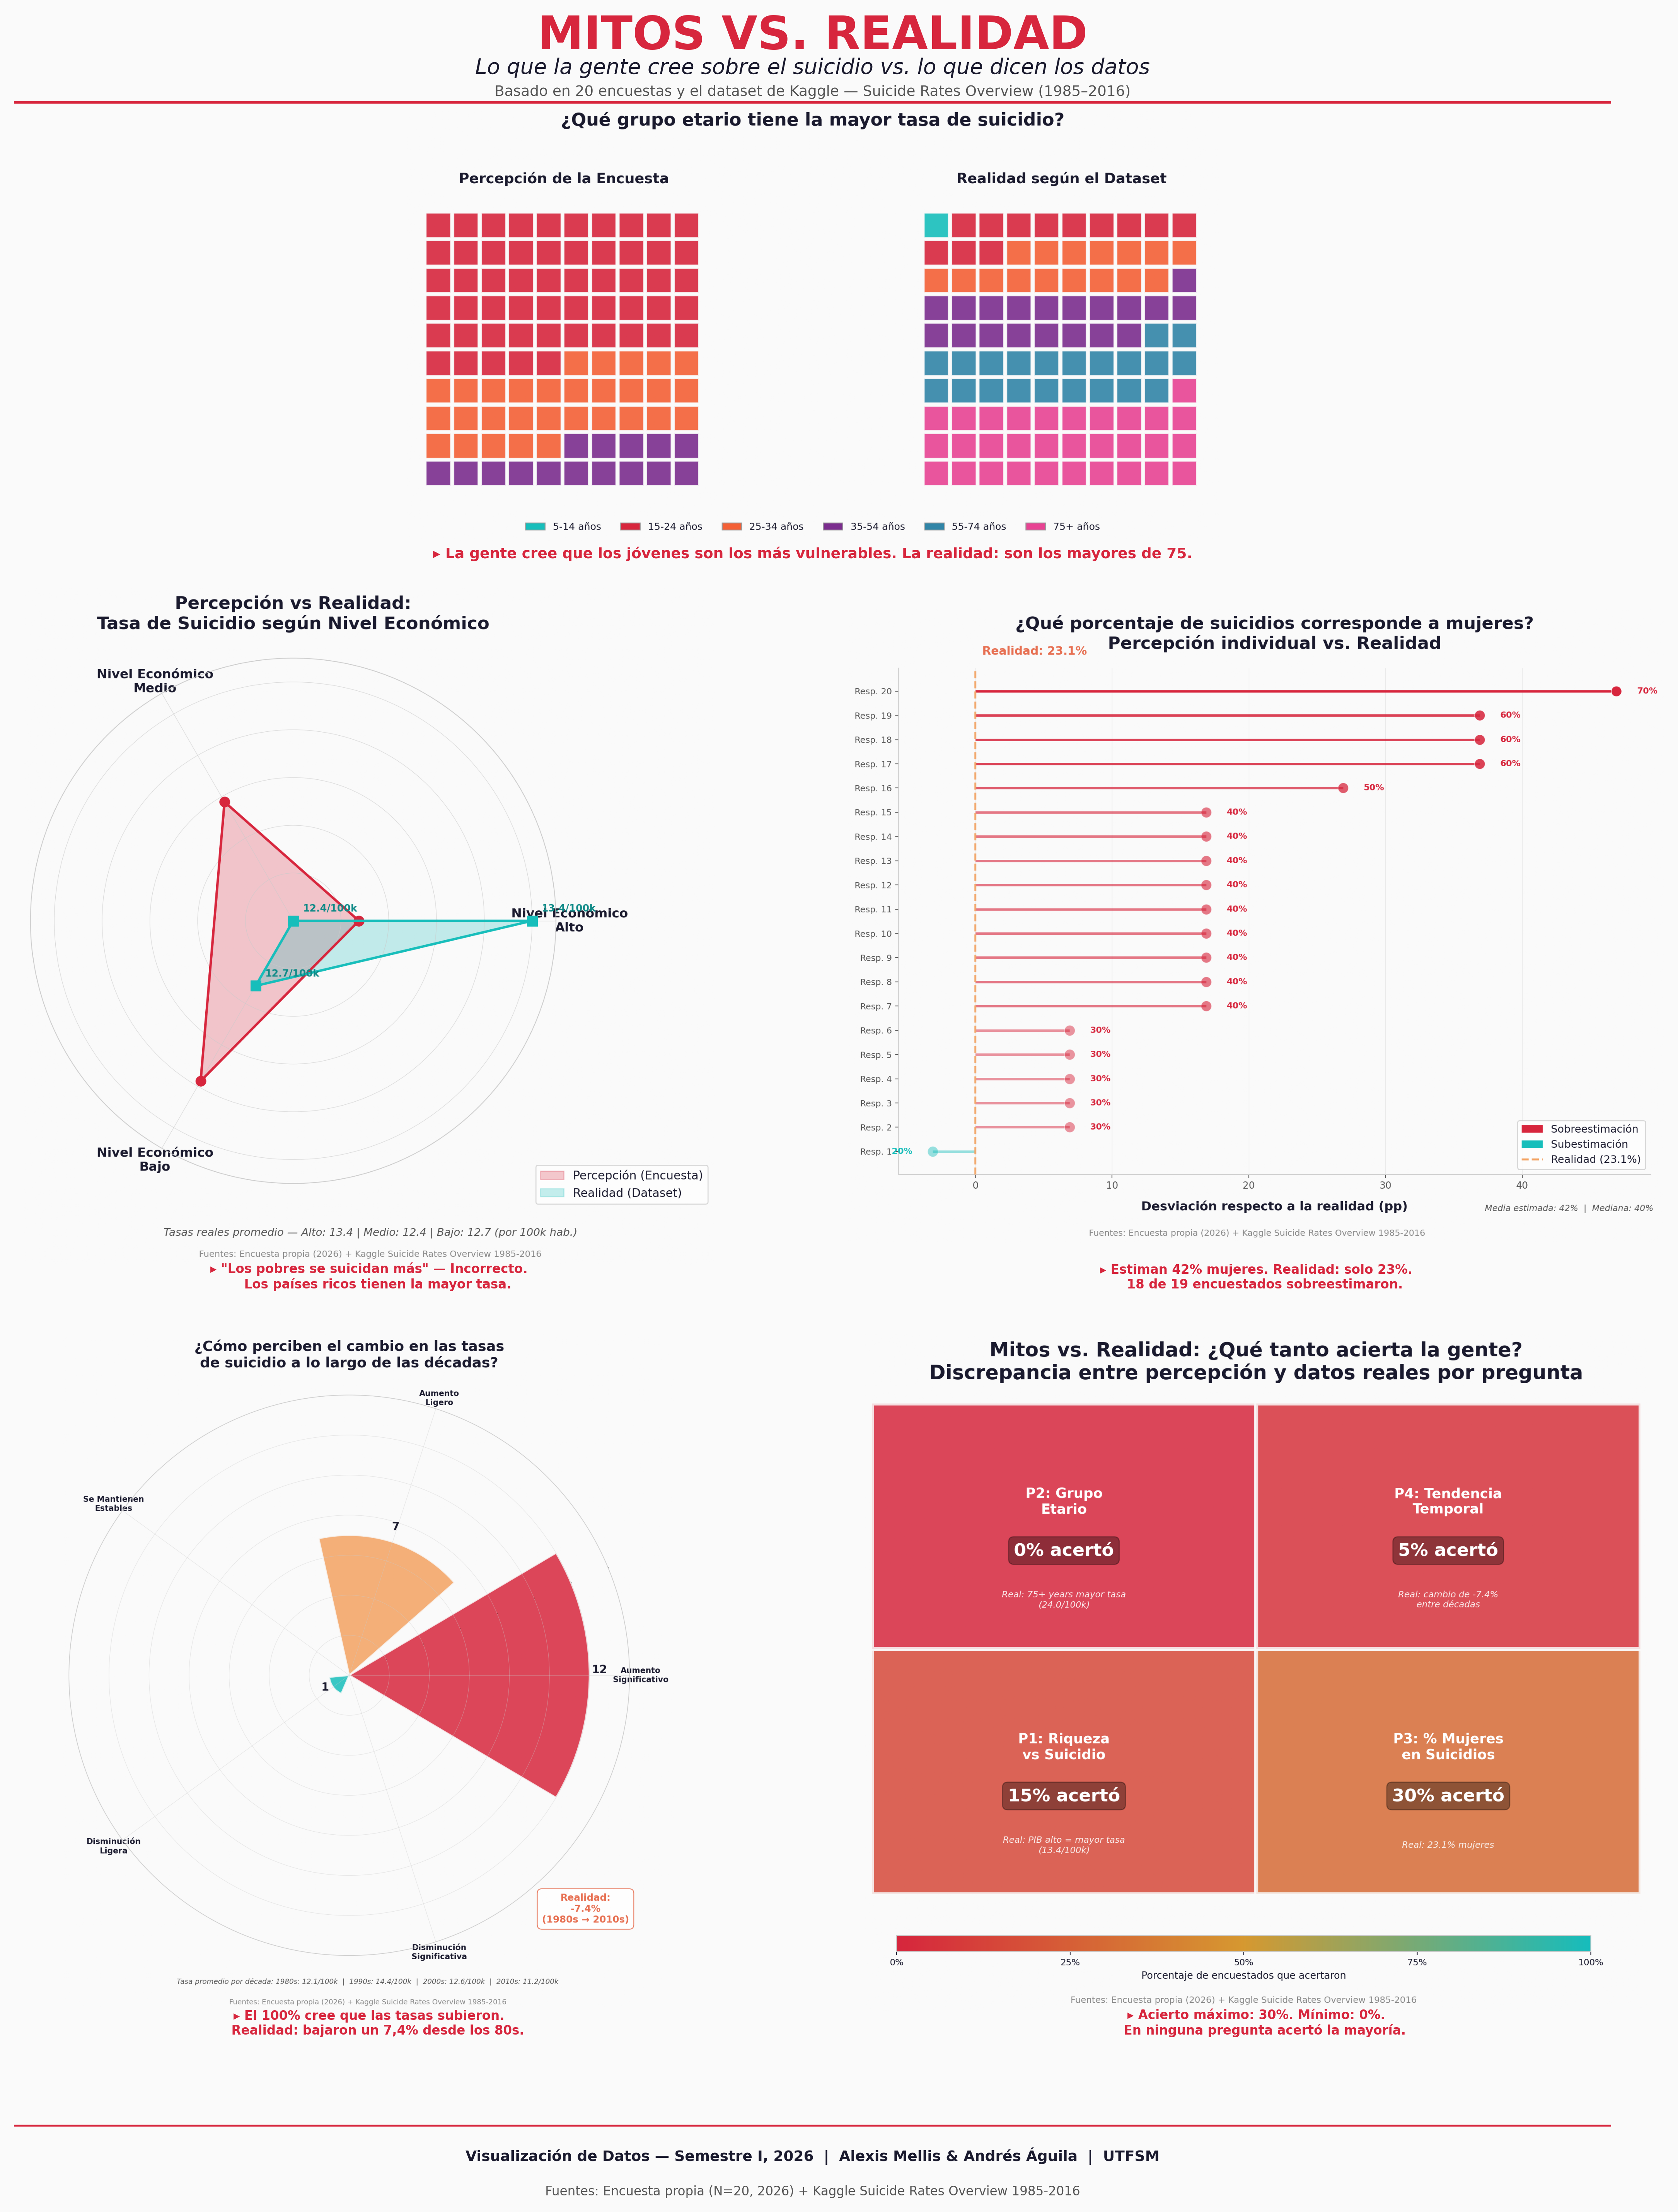
\includegraphics[width=\textwidth]{figures/infografia.png}
  \caption{Infografía grupal. Fuente: Encuesta propia, 2026.}
  \label{fig:infografia}
\end{figure}

% ─────────────────────────────────────────────────────────────────────────────
\section{Trabajo individual -- Integrante 1: Alexis Mellis}

\subsection{Criterios seleccionados}

\begin{enumerate}
  \item \textbf{Criterio A:} % TODO
  \item \textbf{Criterio B:} % TODO
\end{enumerate}

\subsection{Justificación de los criterios}

% TODO: Justificar por qué se eligieron estos criterios.

\subsection{Visualización 1}

\begin{figure}[H]
  \centering
  % 
\includegraphics[width=0.85\textwidth]{figures/figure001.png}
  \caption{TODO: título y fuente.}
  \label{fig:figure001}
\end{figure}

\subsubsection*{Conclusiones}

\begin{itemize}
  \item % TODO
  \item % TODO
  \item % TODO
\end{itemize}

\subsection{Visualización 2}

\begin{figure}[H]
  \centering
  % 
\includegraphics[width=0.85\textwidth]{figures/figure002.png}
  \caption{TODO: título y fuente.}
  \label{fig:figure002}
\end{figure}

\subsubsection*{Conclusiones}

\begin{itemize}
  \item % TODO
  \item % TODO
  \item % TODO
\end{itemize}

% ─────────────────────────────────────────────────────────────────────────────
\section{Trabajo individual -- Integrante 2: Andrés Águila}

\subsection{Criterios seleccionados}

\begin{enumerate}
  \item \textbf{Criterio A:} % TODO
  \item \textbf{Criterio B:} % TODO
\end{enumerate}

\subsection{Justificación de los criterios}

% TODO: Justificar por qué se eligieron estos criterios.

\subsection{Visualización 3}

\begin{figure}[H]
  \centering
  % 
\includegraphics[width=0.85\textwidth]{figures/figure003.png}
  \caption{TODO: título y fuente.}
  \label{fig:figure003}
\end{figure}

\subsubsection*{Conclusiones}

\begin{itemize}
  \item % TODO
  \item % TODO
  \item % TODO
\end{itemize}

\subsection{Visualización 4}

\begin{figure}[H]
  \centering
  % 
\includegraphics[width=0.85\textwidth]{figures/figure004.png}
  \caption{TODO: título y fuente.}
  \label{fig:figure004}
\end{figure}

\subsubsection*{Conclusiones}

\begin{itemize}
  \item % TODO
  \item % TODO
  \item % TODO
\end{itemize}

% ─────────────────────────────────────────────────────────────────────────────
\section{Trabajo grupal -- Visualización con IA generativa}

\subsection{Herramienta utilizada}

% TODO: Indicar la herramienta de IA utilizada (debe ser distinta a la Tarea 1,
%       donde se usó Claude Opus 4.6 via Antigravity).

\subsection{Prompt utilizado}

\begin{lstlisting}[basicstyle=\small\ttfamily, breaklines=true, frame=single]
% TODO: Pegar aqui el prompt utilizado.
\end{lstlisting}

\subsection{Código generado}

\begin{lstlisting}[basicstyle=\small\ttfamily, breaklines=true, frame=single, language=Python]
% TODO: Pegar aqui el código generado por la IA.
\end{lstlisting}

\subsection{Modificaciones realizadas}

% TODO: Describir las modificaciones al código (si no hubo ninguna, indicarlo).

\subsection{Visualización grupal}

\begin{figure}[H]
  \centering
  
\includegraphics[width=0.85\textwidth]{figures/figure001.png}
  \caption{TODO: título y fuente.}
  \label{fig:figure005}
\end{figure}

\subsubsection*{Conclusiones}

\begin{itemize}
  \item % TODO
  \item % TODO
  \item % TODO
\end{itemize}

% ─────────────────────────────────────────────────────────────────────────────
\section{Conclusiones generales}

% TODO: Redactar conclusiones generales integrando los hallazgos
%       de todas las visualizaciones.

% ─────────────────────────────────────────────────────────────────────────────
\section{Repositorio de GitHub}

El código fuente de todas las visualizaciones se encuentra disponible en el siguiente repositorio:

\begin{center}
  \href{https://github.com/siroale/VisualizacionDeDatos-2026-01}{\texttt{https://github.com/siroale/VisualizacionDeDatos-2026-01}}
\end{center}

% TODO: Actualizar la estructura del repositorio con los archivos de la Tarea 2.
\begin{verbatim}
/
|-- Code
|   |-- Agente_IA
|   |   |-- criterio_e_informe.md
|   |   |-- criterio_e.py
|   |-- Alexis-Mellis
|   |   |-- barcode.py
|   |   `-- streamgraph.py
|   `-- Andres-Aguila
|       |-- dumbell.py
|       `-- heatmap.py
|-- Datasets
|   |-- README.md
|   |-- suicide_dataset.csv
|   `-- encuesta.csv
|-- Informe_1
|   |-- figures/
|   |-- informe.pdf
|   `-- informe.tex
|-- Informe_2
|   |-- figures/
|   |-- informe.pdf
|   `-- informe.tex
`-- README.md
\end{verbatim}

% ─────────────────────────────────────────────────────────────────────────────

\end{document}